\section{Theoretische Physik}
\begin{center}

  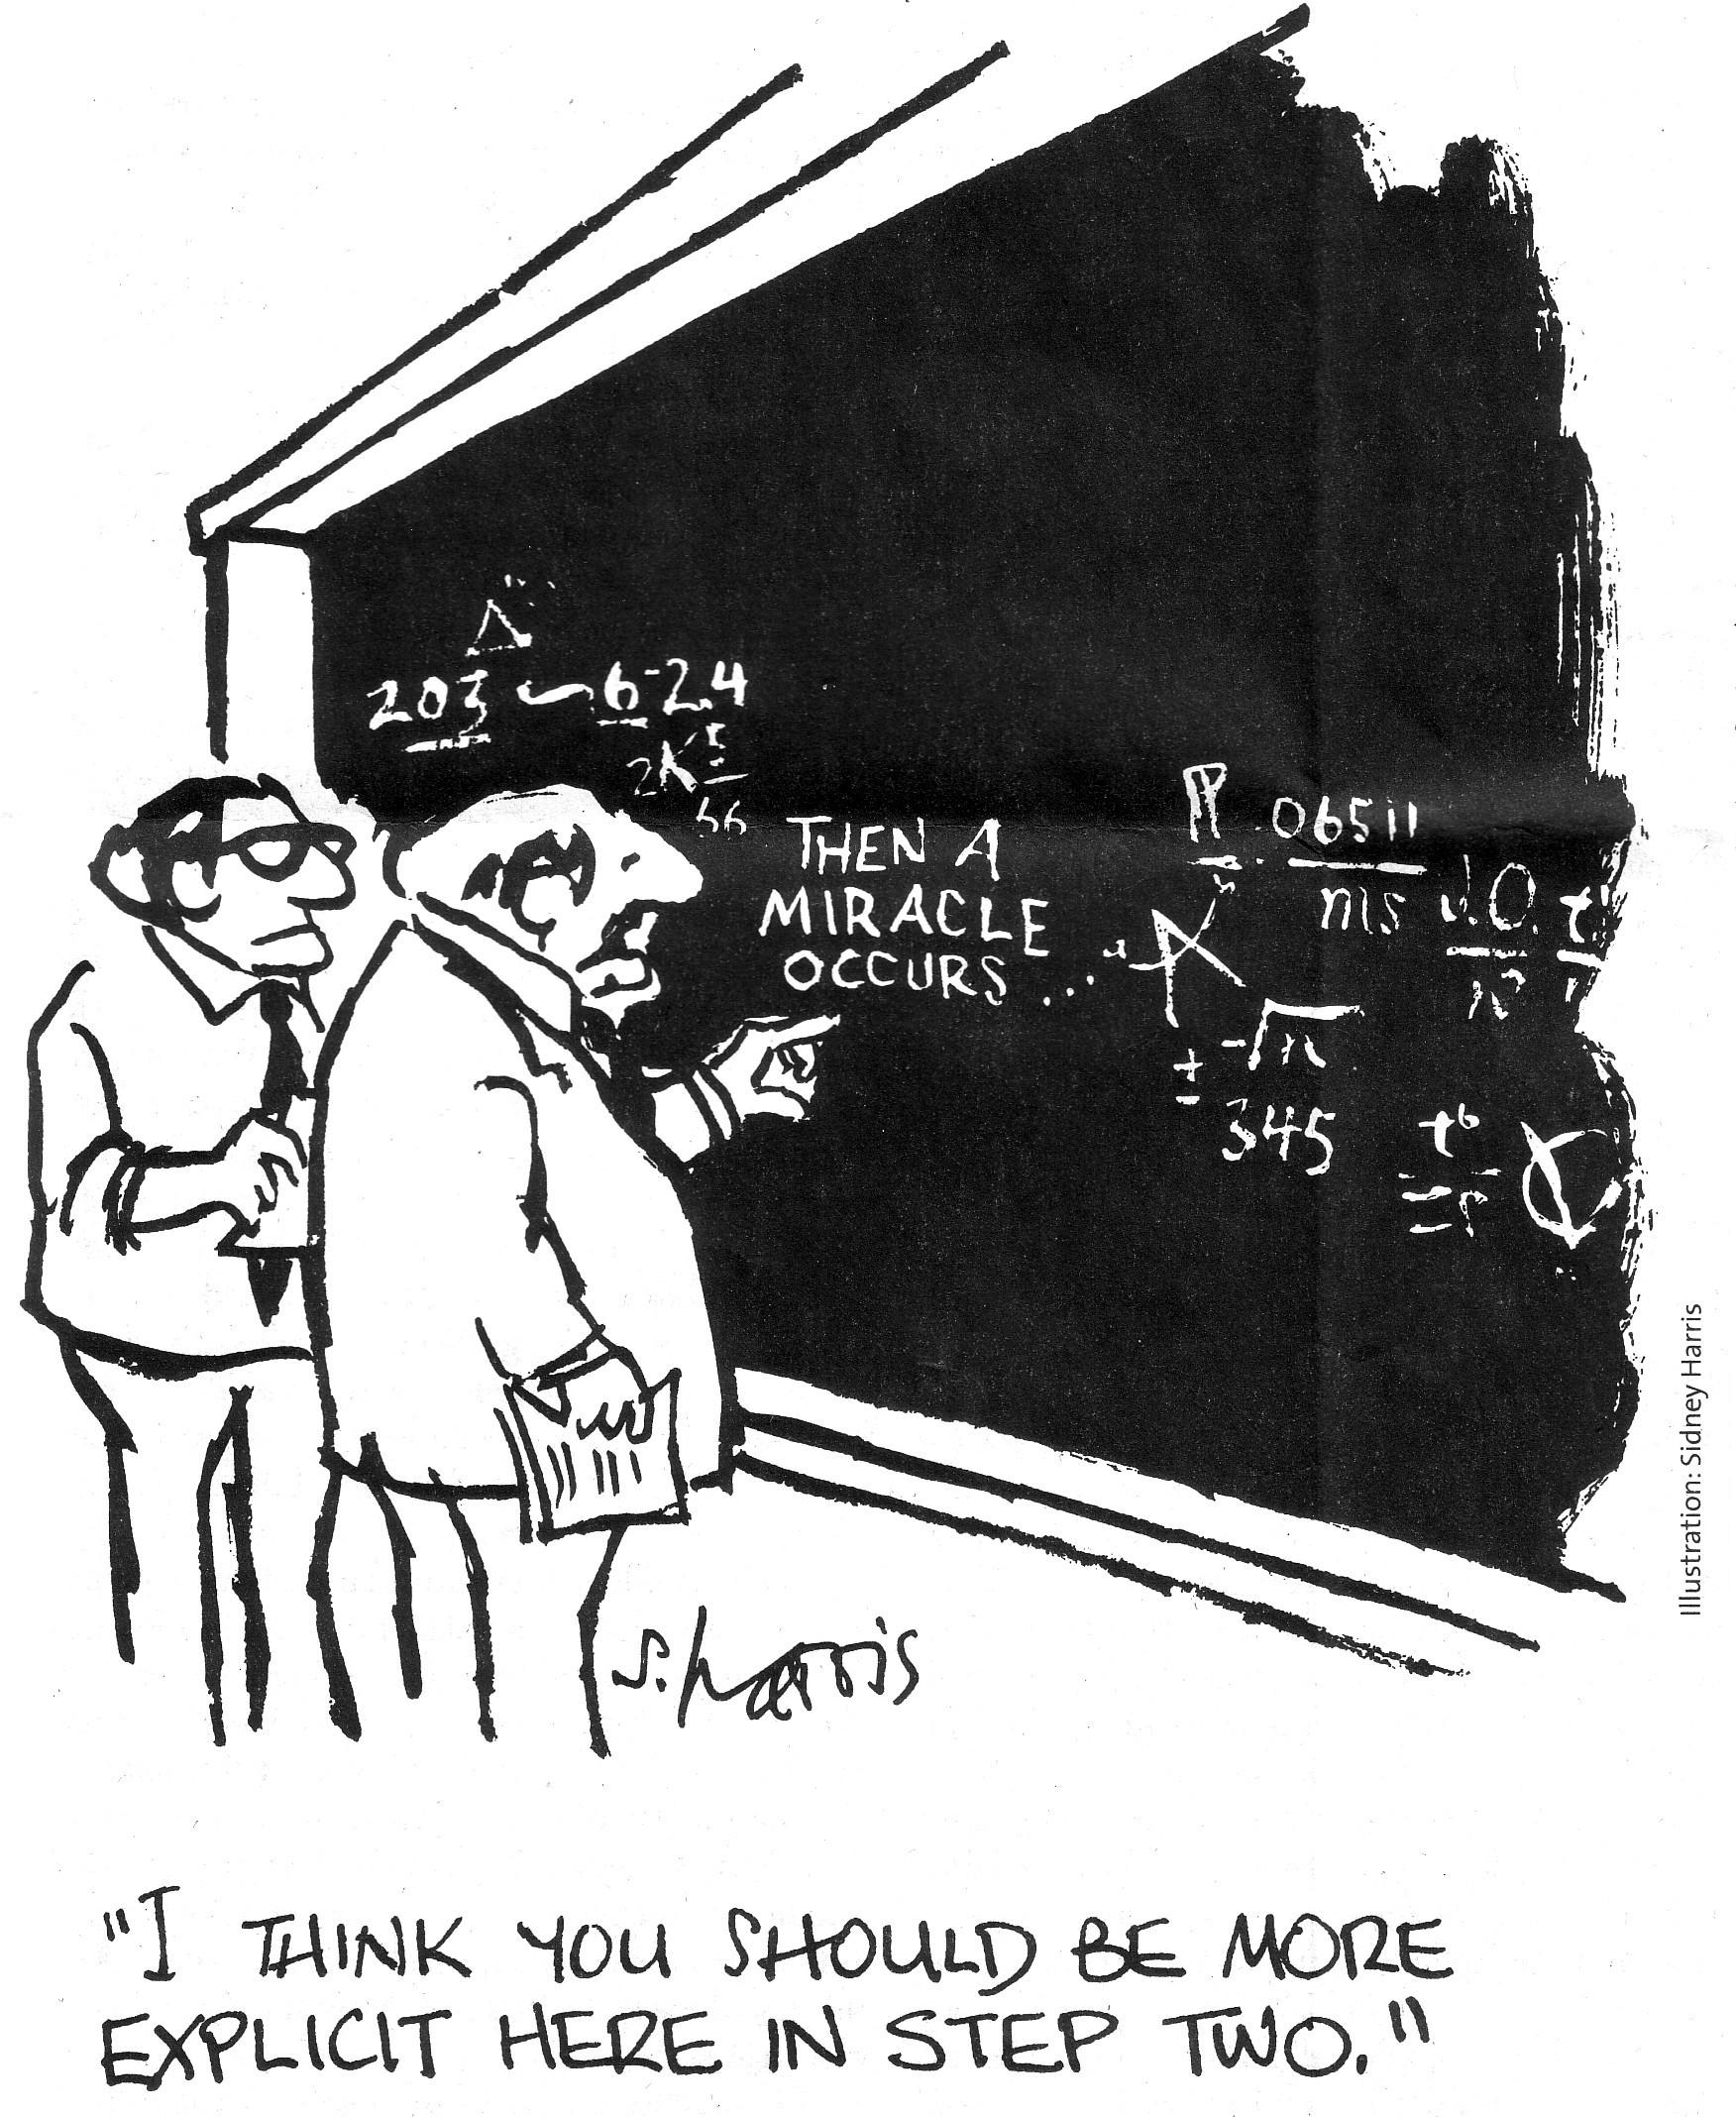
\includegraphics[width=0.2\textwidth]{bilder/miracleoccurs.jpg}

\end{center}
\begin{tabular}{l p{.9\textwidth}}
\textbf{Was:} & Theoretische Physik 1/2: Mathematische Methoden und klassische Mechanik sowie Mathematische Ergänzungen zur Vorlesung\\
\end{tabular}
\rule{\textwidth}{0.1pt}

\textbf{Liebe Erstsemester,} \\
\\
die Sprache der Natur ist die Mathematik und das grundlegende Ziel der Physik ist es, die grundlegenden Naturgesetze in der Form von mathematischen Gleichungen darzustellen. Die theoretische Physik ist das Teilgebiet der Physik, in dem diese mathematischen Gesetze und natürlich auch die Methoden zur Anwendung der Gleichungen auf reale Situationen im Mittelpunkt stehen.
\\
Der Vorlesungszyklus Theoretische Physik I-V entwickelt die Theoretische Physik insgesamt von den Grundlagen bis zu modernen Problemen.
\\
Da Sie Ihr Studium im Sommersemester beginnen, und normalerweise die Vorlesungen im Wintersemester anfangen, haben wir für Sie ein besonderes Programm vorbereitet. Sie können die Vorlesungen theoretische Physik eins und zwei in einem Semester absolvieren. Wegen des großen Aufwands wird die Vorlesung allerdings von zwei Dozenten vorgetragen, Herr Maruhn wird hauptsächlich den physikalischen Anteil präsentieren und einen Teil der mathematischen Methoden dabei entwickeln, und Herr Engel wird die mathematischen Ergänzungen dazu liefern, so dass Sie alles lernen können, was Sie zum Besuch der folgenden Theorievorlesungen benötigen.
\\
Im Mittelpunkt des ersten Teils der Vorlesungen stehen aber die mathematischen Methoden, die für alles weitere grundlegend sind und in der Schule nur selten behandelt werden, vor allem Vektorrechnung, komplexe Zahlen, Funktionen mehrerer Veränderlicher, Differentialgleichungen und Matrizenrechnung.
Diese werden aber immer eng im Zusammenhang mit der Physik behandelt, so dass wir auch einen ersten Überblick über die klassische Mechanik gewinnen werden, wie sie von Galilei und Newton begründet wurde. Die Gesetze der Bewegung von punktförmigen Teilchen in Kraftfeldern werden in verschiedenen Situationen angewendet und führen auch zu so wichtigen Einsichten wie der Erhaltung von Impuls und Energie. Als ein modernes Thema wird auch die spezielle Relativitätstheorie behandelt.
\\
Während dies großen Teils Dinge sind, die Sie von der Schule her kennen, wenn auch nicht so mathematisch fundiert, kommen dann im zweiten Teil der Vorlesung Themen, die Ihnen völlig neu sein sollten: die sogenannte analytische Mechanik nach Lagrange und Hamilton und die Theorie des starren Körpers. Beide sind grundlegend für die moderne theoretische Physik.
\\
In den folgenden Semestern kommen dann die Elektrodynamik, Quantenmechanik und die statistische Mechanik zum Zuge. Ein besonderes Ziel in dieser Folge von Vorlesungen ist es auch, durch immer höhere Abstraktion die Naturgesetze auf wenige universale Prinzipien zurückzuführen, die in allen Gebieten der Physik gleich erscheinen.
\\
Die Mathematik-Kenntnisse, die Sie von der Schule mitbringen, können sehr unterschiedlich sein. Wir werden deshalb in den ersten Übungsstunden Tests durchführen, die nicht bewertet werden und uns einfach einen Überblick über Ihre Vorkenntnisse geben. In der Vorlesung wird dann soviel an Vorkenntnissen angenommen, dass der größte Teil von Ihnen keine Probleme haben sollte. Wenn es doch Anfangsschwierigkeiten gibt, so ist es kein Beinbruch, wenn Sie im Wintersemester noch einmal die Theorievorlesungen im normalen Zyklus beginnen.
\\
Die Übungen sind ein wichtiger Bestandteil der Vorlesung. Jeder, der einmal Stoff aus einem Buch gelernt hat, hat die Erfahrung gemacht, dass es immer noch einen zusätzlichen Schritt erfordert, das Gelernte praktisch anzuwenden. Dabei sollen die Übungen helfen. Für einen Schein ist aktive Mitarbeit in den Übungen und ein Bestehen der Abschlussklausur nötig.
\\
Die Vorlesung kann nur funktionieren, wenn es von Ihnen Feedback gibt. Scheuen Sie sich nicht, Fragen in der Vorlesung zu stellen und auch Kritik zu äußern. Wenn Sie sich dort doch scheuen, können Sie auch die Übungsassistenten ansprechen.

\medskip

Als Literatur empfehle ich
\begin{itemize}
  \item Nolting, Grundkurs Theoretische Physik 1 und 2
  \item Greiner: Mechanik Teil 1und 2
  \item Die Vorlesung wird auch in Form von Tafelbildern und eines Skriptes im Rahmen des eLearning-Portals ILIAS ins Internet gestellt.
\end{itemize}

\noindent
Zur Mathematik gibt es eine große Auswahl.
Empfehlenswert einfach ist:
May-Britt Kallenrode: Rechenmethoden der Physik: Mathematischer Begleiter zur Experimentalphysik\\
Diese Bücher sind teilweise auch als eBooks über die Universitätsbibliothek beziehbar.
Auch das Skript für die mathematischen Ergänzungen wird im Rahmen des eLearning-Portals ILIAS im Internet verfügbar sein.\\
\\
\noindent

Wir wünschen Ihnen viel Spaß und Erfolg im Physikstudium!\\
\begin{flushright}
Joachim Maruhn und Eberhard Engel
\end{flushright}

